\chapter{Systemmodelle}


\section{Interaktionsverlauf}

Menüeinträge:

\begin{longtable}{|p{0.25\textwidth}|p{0.75\textwidth}|}
    \hline
    main menu & Das ist die erste Ansicht, die der Nutzer bekommt. Von hier aus erreicht er alle Bereiche des Programms.\\
    
    \hline
    
    creative & Von hier aus startet der Nutzer ein neues Spiel, mit einem einfachem Standardknoten, lädt einen Speicherstand oder startet das erstellen von neuen Herausforderungen (challenges).\\
    
    \hline
    
    challenge & Eine Übersicht, der vorhandenen Herausforderungen. Der Nutzer kann nach verschieden Kriterien suchen und sortieren lassen und in einer Vorschau weitere Informationen betrachten.\\

    \hline
    
    settings & Einstellungen an Grafik, Ton und Steuerung. Außerdem kann die persönliche Farbpalette angepasst werden.\\

    \hline
    
    credits & Zeigt Infos über die Mitwirkenden an dem Programm und über das Programm selber.\\

    \hline
    
   \end{longtable}
    
	\begin{figure}[h]
	  \centering
	  \includesvg[svgpath=Systemmodelle/, width = 12.5cm]{menu}
	  %\caption{...}
	\end{figure}
	~\\
	Im Spiel kann der Nutzer auch die {\color{red} Einstellungen} erreichen. Die Menüeinträge in den unterschiedlichen Spielmodi können variieren.
	settings - Genau wie aus dem Hauptmenü.
	save - Speichert den aktuellen Spielstand.
	quit - Beendet das laufende Spiel.
	render options - Bietet dem Nutzer verschiedene Möglichkeiten seinen Knoten zu rendern und zu exportieren.
    \begin{figure}[htbp]
	  \centering
	  \includesvg[svgpath=Systemmodelle/, width = 5cm]{ingamemenu}
	  %\caption{...}
	\end{figure}


\section{Benutzerinteraktionsmodelle}

	\begin{figure}[htbp]
	  \centering
	  \includesvg[svgpath=Systemmodelle/, width = \textwidth]{Spielverlauf}
	  %\caption{...}
	\end{figure}
	
\subsection{Ungültige Züge}

	\begin{figure}[htb]
	  \centering
	  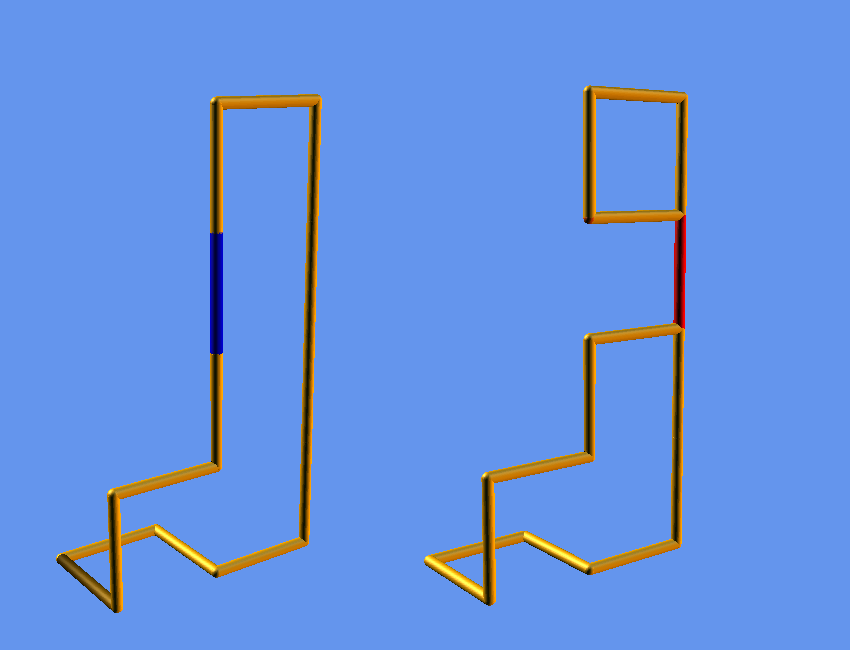
\includegraphics[width = \textwidth]{Systemmodelle/Ungueltiger_Zug.png}
	  \caption{...}
	  \label{fig:zug1}
	\end{figure}

Der Knoten auf der linken Seite \ref{fig:zug1} beschreibt eine gültige Spielsituation. Der Spieler wählt eine Kante (blaue Hervorhebung) aus, um einen weiteren Zug vorzunehmen.
Einem Spieler ist es nicht möglich, zwei parallele Kanten (hier: die Blaue und die Rote) zu einer Kante zu vereinen. Der Knoten soll immer aus einem geschlossenen Kreis von Kanten bestehen. Der Knoten auf der rechten Seite \ref{fig:zug1} ist daher eine ungültige Spielsituation.



\section{Benutzerschnittstelle}

%	\begin{figure}[htbp]
%	  \centering
%	  \includesvg[svgpath=Systemmodelle/, width = \textwidth]{Hauptmenue_grob_entwurf}
%	  %\caption{...}
%	\end{figure}
%
%	\begin{figure}[htbp]
%	  \centering
%	  \includesvg[svgpath=Systemmodelle/, width = \textwidth]{Auswahl}
%	  %\caption{...}
%	\end{figure}
